
\chapter{Experimental Results}
\label{chap:exp}

This chapter presents the experiments and the results when it comes to the evaluation of the following methods. A propose robot-camera calibration method and the 3D object pose estimation method. As to the robot-camera calibration method, the internal parameters of the camera to be calibrated need to be estimated. Methods for estimating the internal parameters also known as intrinsic parameters of the camera already exists and two of the most popular methods available in the open source community were selected. A detail description of those methods is in \ref{chap:robot}. In order to validate the output of the methods, a reprojection error as standar metric is selected in this thesis. Then, with the most accurate internal parameters, the camera-robot calibration proceeds. A repeattability test, as validation test for the result of the robot-camera calibration  follows. And finally, with the most accurate result of the robot-camera calibration, experiments for testing the 3D pose estimation system follows. For the purpose of testing, an industrial object is required as well as its CAD model. The later is accomplised with use of the FreeCAD software \ref{freecadb}, then, a suitable scaling undergoes with the use of CluodCompare software \ref{cloudcompareb}, where a point cloud is generated. As to the validation of the method, a ground truth of the object needs to be known in advance. For such a requirement. A checkboard is used as described in Figure \ref{setupsystem}. Then, by placing the robot TCP to the specific points (three points in totally), the checkerboard can be localized. With that, a new workspace is produced.By analizing the translation and rotation erros the system is evaluated.\\
The checkboard workspace is used for a roughly estimation of the object's pose wich is compare with 3D object pose estimation system described in \ref{chap:theo}.  


\section{Robot-Camera Calibration on the Yumi robot}
In order to get an accurate estimation of the robot-camera pose depends on how well the estimation of the intrinsic parameters related to the camera can be. Such estimation of those parameters was accomplished as described in section \ref{pppp}, where those existing algorithms were used for checkerboard detection in both colour and depth data. With those parameter knowing in advance, a reprojection error is calculated for both cameras. 

\subsubsection{Reprojection Error}

The reprojection error is the distance between a pattern keypoint detected in a calibration image, and a corresponding world point projected into the same image. Figure \ref{fig:realopen} and Figure \ref{fig:realros} show the calibration results by analyzing the reprojection error per image for the RealSense camera when OpenCV and camera \textunderscore industrial calibration were used. Figure \ref{fig:astraopen} and Figure \ref{fig:astraros} show the calibration results by analyzing the reprojection error per image for the Astra camera when the OpenCV and camera \textunderscore industrial calibration were used.
%%%%%%%%%%%%%%%%%%%%%%%%%%%%%%%%%%%%%%%%%%
\begin{figure}[!h]
\begin{center}
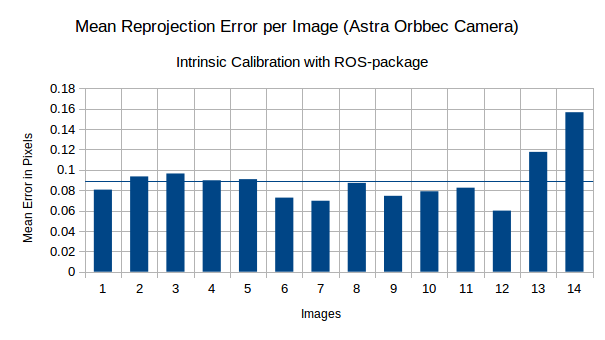
\includegraphics[width=5in, height=3.5in]{figures05/ros_int_cal_astra.png}
\caption{Mean Reprojection Error per image with a ROS method (Astra Orbbec Camera)}%\cite{temp2}}
\label{fig:astraros}
\end{center}
\end{figure}

\begin{figure}[!h]
\begin{center}
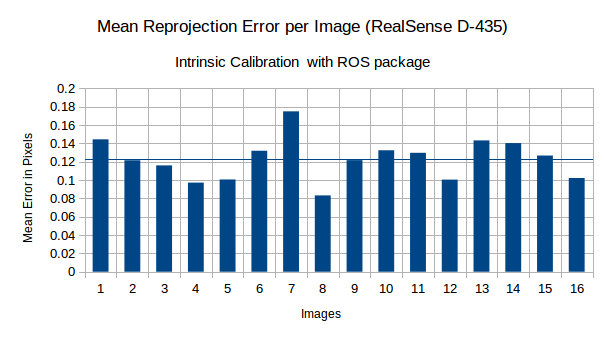
\includegraphics[width=5in, height=3.5in]{figures05/ros_int_cal_real.png}
\caption{Mean Reprojection Error per image with a ROS method (RealSense D-435)}%\cite{temp2}}
\label{fig:realros}
\end{center}
\end{figure}

\begin{figure}[!h]
\begin{center}
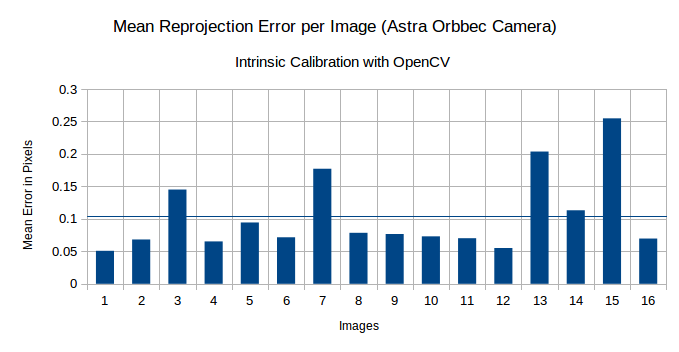
\includegraphics[width=5in, height=3.5in]{figures05/opencv_int_cal_astra.png}
\caption{Mean Reprojection Error per image with a OpenCV method (Astra Orbbec Camera)}%\cite{temp2}}
\label{fig:astraopen}
\end{center}
\end{figure}

\begin{figure}[!h]
\begin{center}
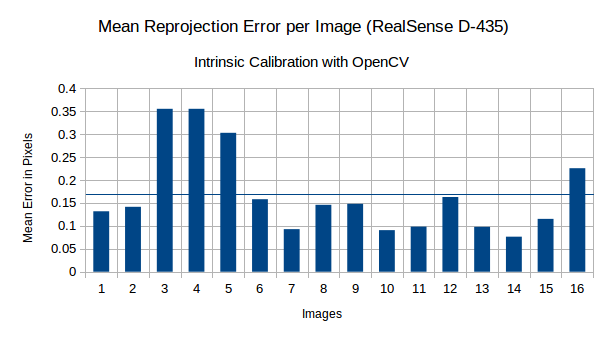
\includegraphics[width=5in, height=3.5in]{figures05/opencv_int_cal_real.png}
\caption{Mean Reprojection Error per image with a OpenCV method (RealSense D-435)}%\cite{temp2}}
\label{fig:realopen}
\end{center}
\end{figure}

To find the average error we calculate the arithmetical mean of the errors calculates for all the calibration images. This should be as close to zero as possible. 

\subsubsection{Result Analysis}
After computing the average error for both cameras, the results are shown in Table \ref{astra1} related to the Astra camera and Table \ref{real1} which corresponds to the RealSense D-435. It can be seen that the overall mean error representing the Astra camera is quite correlated to one another method (OpenCV or camera \textunderscore industrial calibration). The difference is acceptable since it is under the standard specified in most of the literature of computer vision as it is that the error should as close as possible to 0, or under the 0.5 pixels.\\
On the other hand, the results for the RealSense camera are not quite correlated at all. There exists a difference that can affect the eye-to-hand calibration process, and therefore, the pose estimation system can be affected also. Even when the overall mean error meets the requirements of being under the 0,5 pixels, it is difficult to conclude that the RealSense camera is or is not a good choice for solving the main problem of this thesis as it is the pose estimation system. But, it is a good insight to know in advance for future conclusions where there might exist potential issues in the development of this master thesis.
As a remark, both cameras were calibrated with same light conditions, with the same calibration target and with an equal number of images. Considering, all in all, it can be concluded that the Astra camera seems to perform well and it can be our final choice for the pose estimation system.

\begin{table}[b]
% increase table row spacing, adjust to taste
\renewcommand{\arraystretch}{1.3}
\caption{Experiment data for internal Astra sensor calibration.}
\label{astra1}
\centering
\begin{tabular}{|c||c|}
\hline
Method & Overall Mean Error\\
\hline
OpenCV &  0.1041954808\\
\hline
ROS &  0.1081118023\\
\hline
\hline
\end{tabular}
\end{table}

\begin{table}[b]
% increase table row spacing, adjust to taste
\renewcommand{\arraystretch}{1.3}
\caption{Experiment data for internal RealSense sensor calibration.}
\label{real1}
\centering
\begin{tabular}{|c||c|}
\hline
Method & Overall Mean Error\\
\hline
OpenCV &  0.1684388411\\
\hline
ROS &  0.122868849\\
\hline
\hline
\end{tabular}
\end{table}

\subsection{Eye-To-Hand Calibration}
The second experiment in this chapter is related to the eye-to-hand calibration. In this experiment, the Astra and RealSense cameras were used. Since, the quality of the extrinsic parameters depends on how good the estimation of the intrinsic parameters are, the internal parameters were selected carefully by analizing the reprojection error of each individual camera as mentioned previously. The less reprojection error the camera produces, the more accurate the camera is. \\
By defining the most accurate internal parameter for each one of the camera respectively. The experiment to be performed are divided in two types.
In the first type of experiment, where the calibration plate is kept at a constant angle, parallel to the XY plane of the robot coordinate system as it is shown in Figure \ref{iiiii}, the robot proceed with execution of several predefined set of movements (translation) around the XY plane.\\ 
As to the second experiment, where the calibration plate is   tilting with predefined orientations and small translation around the XY plane of the robot frame, provided that the checkboard is always detected by the camera to be calibrated the robot execute the movement. In between of the movements, a pause is set in order to let the camera take a good quality of 2D image that later is used for the pose estimation of the camera.\\

In order to excute the movement of the robot arm and compute the estimation of the camera frame relative to the robot frame, three nodes were developed as described in \ref{jjjjjj}, where one of the node is for controlling the robot movement and publishing the transformation from the robot base frame to TCP (Tool Center Point) frame in the ROS network (tf topic to be specific). While the other node is for estimating the pose of the camera relative the to the calibration target frame and braodcasting this pose in the ROS networke. When it comes to the last node, which is responsible for keeping track of the all coordinate frames over time, and querying for the transformation of the camera frame relative to the robot frame. In addition to that, an average transformation is computed after each executed movement of the robot arm. Since the quality of robot-camera pose depends on the quality of the image taken, a pause of few seconds between movements in the robot control node is set in order to cancel the effects of possible vibrations that the robot can produce, so that wrong measurements are avoided.



\subsubsection{Calibration results}


%%%%%%%%%%%%% astra 




\begin{itemize}
\item The following eye-to-hand transform was obtained for the Astra Camera with the calibration plate parallel to the XY plane in robot frame:
\begin{equation}
^{R}T_{C}=\begin{bmatrix} -2.26051005e-02 & 7.30112611e-01 & -6.82952842e-01 & 1.19260379\\9.99481127e-01 & 8.25583772e-04 & -3.21992981e-02 & 0.12098781\\ -2.29452788e-02 & -6.83326345e-01 & -7.29752438e-01 & 0.53569317 \end{bmatrix}
\end{equation}


				
\item The following eye-to-hand transform was obtained for the Astra Camera by tilting the calibration plate:
\begin{equation}
^{R}T_{C}=\begin{bmatrix} -0.01440125 & 0.72431469 & -0.68931911 & 1.19518608\\0.99970886 & -0.00291747 & -0.02395149 & 0.11374275\\ -0.01935949 & -0.68946336 & -0.7240618 & 0.53606583 \end{bmatrix}
\end{equation}


%%%%%%%%%%%%%%%%% realsense

\item The following eye-to-hand transform was obtained for the RealSense D-435 camera with the calibration plate parallel to the XY plane in robot frame:
\begin{equation}
^{R}T_{C}=\begin{bmatrix} -2.23312402e-02 & 2.94145863e-01 & -9.55499622e-01 &1.22253213\\9.99723971e-01 & -4.09078692e-04 & -2.34907523e-02 & 0.11776472 \\ -7.30058216e-03 & -9.55760453e-01 & -2.94055535e-01 & 0.32424239  \end{bmatrix}
\end{equation}



\item The following eye-to-hand transform was obtained for the RealSense D-435 camera by tilting the calibration plate:
\begin{equation}
^{R}T_{C}=\begin{bmatrix} -0.01833338  0.30085851 -0.95349255 & 1.21972025\\0.99978158 -0.00405373 -0.02050249& 0.09386797\\ -0.01003355 -0.95366017 -0.30071848& 0.33192816\end{bmatrix}
\end{equation}
\end{itemize}


\subsubsection{Result Analysis}

The propose robot-camera calibration method was successfully performed provided that the calibration target was detected by the 3D camera to be calibrated. In order to validate whether the propose method is accurate enough for the pose estimation system discribed in \ref{oooooo} or not, a ground truth is neccesary to know in advance. But it was a challenging task to meassure an exact orientation and translation of the camera with respect to the robot frame. One of the several diffulties encounter was that the housing of the camera (namely the RealSense camera) is rounded which makes it hard to get good measurement of the mounting point to the camera. Another issue, the robot and the set of cameras were mounting on different tables such that a simple meassurement of distance was not possible to do it with a reasonable accuracy. In addition to that, the rotation of the sensor in the housing is also not known. A simple solution would be to use an industrial camera where knowing transformations are available. But this was not available. \\
The propuse solution needed to be evaluated somehow. Since a traditional error estimation for evalution is not possible, in this thesis a repeatability test is taken into account for the evalutation. The repeatability test consiste of run again the robot but with the major difference that the number of movements is increased. In addition that, the orientation and displacement of the calibration target are modified for each individual movement also. By doing the repeatability test an average translation and orientation is presented in \ref{uuu}.












%For Astra Camera

\begin{table}[b]
\renewcommand{\arraystretch}{1.3}
\caption{Mean Values of The Repeatability Test With a Constant Orientation of the Calibration Plate(Astra Camera).}
\label{meanastra1}
\centering
\begin{tabular}{|c||c||c||c||c||c||c|}
\hline
$x[m]$ & $y[m]$ & $z[m]$ & $q_{x}$ & $q_{y}$ & $q_{z}$ &$q_{\omega}$ \\
\hline
1.1926 & 0.1245 & 0.5368& 0.653175&	0.661978&	-0.269761&	-0.249755 \\
\hline
\hline
\end{tabular}
\end{table}

\begin{table}[b]
\renewcommand{\arraystretch}{1.3}
\caption{Standar Deviation from The Repeatability Test With a Constant Orientation of the Calibration Plate(Astra Camera).}
\label{standarastra1}
\centering
\begin{tabular}{|c||c||c||c||c||c||c|}
\hline
$\sigma_{x[m]}$ & $\sigma_{y[m]}$ & $\sigma_{z[m]}$ & $\sigma_{q_{x}}$ & $\sigma_{q_{y}}$ & $\sigma_{q_{z}}$ &$\sigma_{q_{\omega}}$ \\
\hline
0.011012&	0.009877	&0.000906&0.000243&	8.45E-05&	0.000446&	0.000976\\
\hline
\hline
\end{tabular}
\end{table}


\begin{table}[b]
\renewcommand{\arraystretch}{1.3}
\caption{Mean Values of The Repeatability Test With Tilting Motion of the Calibration Plate(Astra Camera).}
\label{meanastra2}
\centering
\begin{tabular}{|c||c||c||c||c||c||c|}
\hline
$x[m]$ & $y[m]$ & $z[m]$ & $q_{x}$ & $q_{y}$ & $q_{z}$ &$q_{\omega}$ \\
\hline
1.197089&	0.116571&	0.539509&
0.653488&	0.660281&	-0.270449&	-0.252499 \\
\hline
\hline
\end{tabular}
\end{table}


\begin{table}[b]
\renewcommand{\arraystretch}{1.3}
\caption{Standar Deviation from The Repeatability Test With Tilting Orientation of the Calibration Plate(Astra Camera).}
\label{standarastra2}
\centering
\begin{tabular}{|c||c||c||c||c||c||c|}
\hline
$\sigma_{x[m]}$ & $\sigma_{y[m]}$ & $\sigma_{z[m]}$ & $\sigma_{q_{x}}$ & $\sigma_{q_{y}}$ & $\sigma_{q_{z}}$ &$\sigma_{q_{\omega}}$ \\
0.012046&	0.010473&	0.008465& 0.000837&	0.002155&	0.000920&	0.002450
\\
\hline
\hline
\end{tabular}
\end{table}



%For Real Sense Camera
\begin{table}[b]
\renewcommand{\arraystretch}{1.3}
\caption{Mean Values of The Repeatability Test With a Constant Orientation of the Calibration Plate(RealSense Camera).}
\label{meanreal1}
\centering
\begin{tabular}{|c||c||c||c||c||c||c|}
\hline
$x[m]$ & $y[m]$ & $z[m]$ & $q_{x}$ & $q_{y}$ & $q_{z}$ &$q_{\omega}$ \\
\hline
1.222425&	0.112532&	0.324441&0.564006&	0.573552&	-0.426780&	-0.413272 \\
\hline
\hline
\end{tabular}
\end{table}


\begin{table}[b]
\renewcommand{\arraystretch}{1.3}
\caption{Standar Deviation from The Repeatability Test With a Constant Orientation of the Calibration Plate(RealSense).}
\label{standarreal1}
\centering
\begin{tabular}{|c||c||c||c||c||c||c|}
\hline
$\sigma_{x[m]}$ & $\sigma_{y[m]}$ & $\sigma_{z[m]}$ & $\sigma_{q_{x}}$ & $\sigma_{q_{y}}$ & $\sigma_{q_{z}}$ &$\sigma_{q_{\omega}}$ \\
\hline
0.000160&	0.007729&	0.000294&9.20E-05&	4.19E-05&	5.26E-05&	1.31E-05\\
\hline
\hline
\end{tabular}
\end{table}


\begin{table}[b]
\renewcommand{\arraystretch}{1.3}
\caption{Mean Values of The Repeatability Test With Tilting Motion of the Calibration Plate(Real Sense).}
\label{meanreal2}
\centering
\begin{tabular}{|c||c||c||c||c||c||c|}
\hline
$x[m]$ & $y[m]$ & $z[m]$ & $q_{x}$ & $q_{y}$ & $q_{z}$ &$q_{\omega}$ \\
\hline
1.198174&	0.114574&	0.530653& 0.653669&	0.660107&-0.270259&	-0.252684 \\
\hline
\hline
\end{tabular}
\end{table}

\begin{table}[b]
\renewcommand{\arraystretch}{1.3}
\caption{Standar Deviation from The Repeatability Test With Tilting Orientation of the Calibration Plate(RealSense Camera).}
\label{standarreal2}
\centering
\begin{tabular}{|c||c||c||c||c||c||c|}
\hline
$\sigma_{x[m]}$ & $\sigma_{y[m]}$ & $\sigma_{z[m]}$ & $\sigma_{q_{x}}$ & $\sigma_{q_{y}}$ & $\sigma_{q_{z}}$ &$\sigma_{q_{\omega}}$ \\
0.010322&	0.012213&	0.020068&			0.000893&	0.002086&	0.000676&	0.002326\\
\hline
\hline
\end{tabular}
\end{table}



\section{Pose Estimation Pipeline}
